\documentclass[12pt]{article}
 
\usepackage[margin=1in]{geometry} 
\usepackage{amsmath,amsthm,amssymb,outlines}
\usepackage{graphicx}
\usepackage{tikzsymbols}
\newenvironment{statement}[2][Statement]{\begin{trivlist}
\item[\hskip \labelsep {\bfseries #1}\hskip \labelsep {\bfseries #2.}]}{\end{trivlist}}

\begin{document}
 
\title{MATH 8200 Homework 4} 
\author{}
\maketitle

\begin{statement}[Problem]{1}
  Show that the complement of a finite set of points in $\mathbb{R}^n$ is simply-connected if $n \geq 3$. 
\end{statement}
\begin{proof}
  (Note that the following pictures are only for the $n=3$ case, but a similar idea is followed for $n >3$.) We begin by imagining these $n$ missing points in an $nth$ dimensional elipsoid-like shape:
  \par \begin{center} 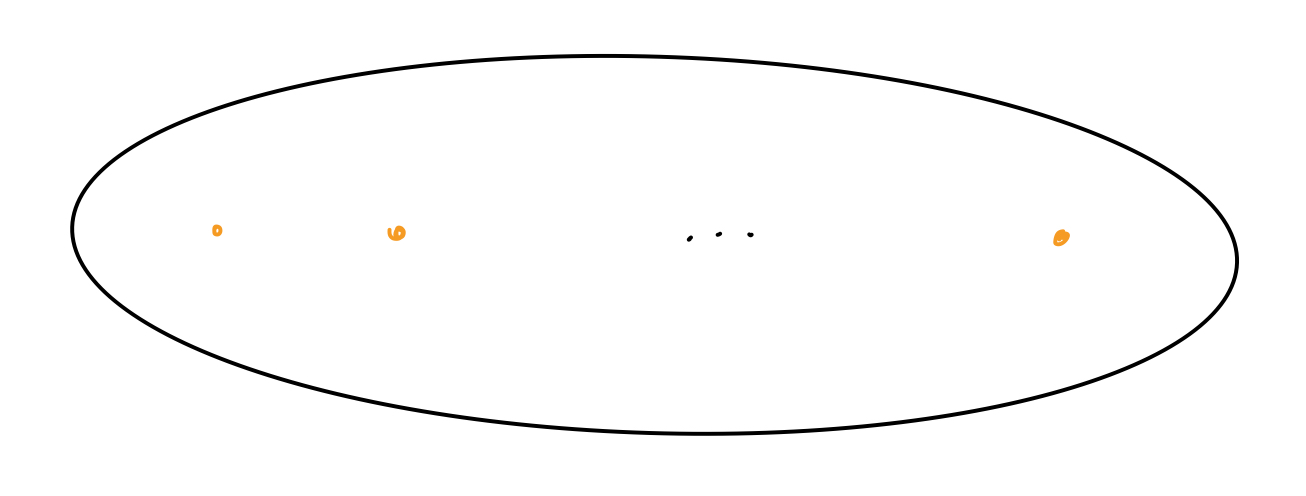
\includegraphics[scale=.2]{1-1.jpg} \end{center}
  \par From here, we can "pinch" in between the $n$ missing points to create $n$ $D^n$'s, each missing a point in the center.
  \par \begin{center} 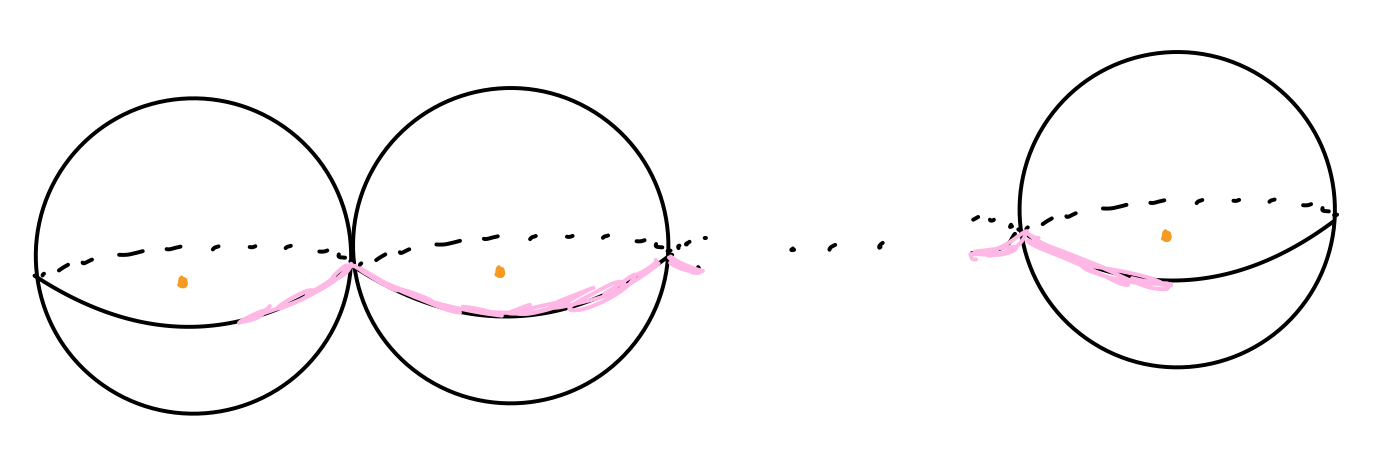
\includegraphics[scale=.2]{1-2.jpg} \end{center}
  \par Then, note that the pink line continues on the boundary of all $n$ $D^n$'s, and can be contracted to a point. 
  \par \begin{center} 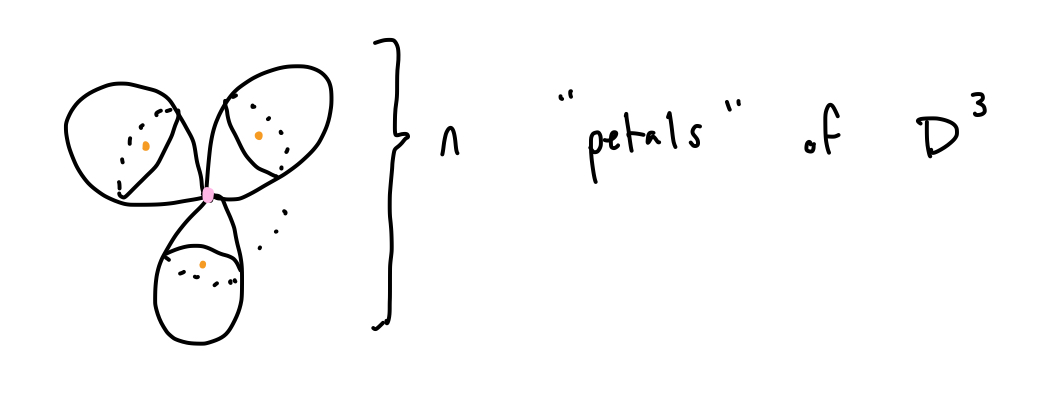
\includegraphics[scale=.2]{1-3.jpg} \end{center}
  \par Then, in each $D^n$, the hole in the center can be expanded so that together the $D^n$ and the hole become an $S^{n-1}$.
  \par \begin{center} 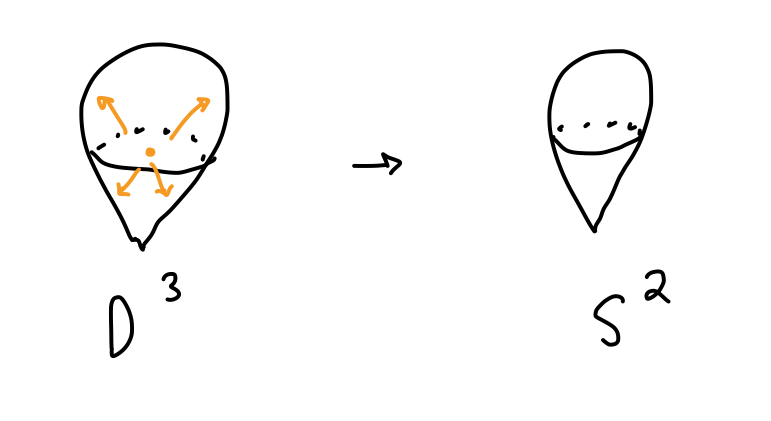
\includegraphics[scale=.2]{1-4.jpg} \end{center}
  \par \begin{center} 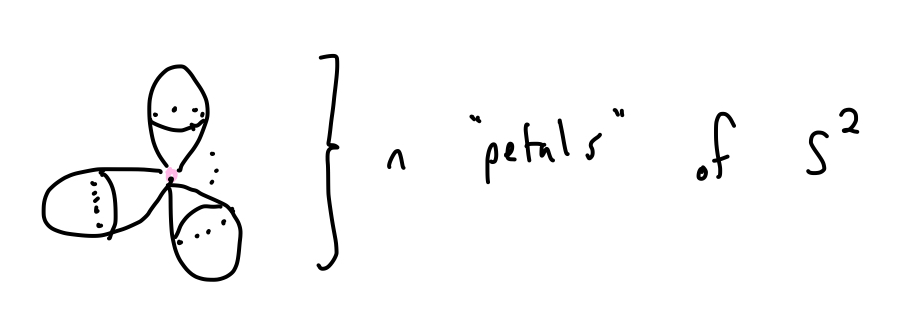
\includegraphics[scale=.2]{1-5.jpg} \end{center}
  \par This is clearly path connected, as this is a wedge sum of $n$ $S^{n-1}$'s. Then, because the fundamental group of $S^n$ is trivial for $n \geq 2$, we know 
 \begin{align*}
   \pi_1( \mathbb{R}^n / \{x_0, x_1, \dots, x_n\}) & \cong \pi_1(\vee^n(S^{n-1})) \\
                                                   & \cong \pi_1(S^{n-1}) \ast \dots \ast \pi_1(S^{n-1}) \\ 
                                                   & \cong 0 \ast \dots \ast 0 \\
                                                   & \cong 0.
 \end{align*}
 Thus the space is path connected and has a trivial fundamental group, so it is simply-connected.
\end{proof}

\begin{statement}[Problem]{2}
  Let $X \subset \mathbb{R}^3$ be the union of $n$ lines through the origin. Compute $\pi_1(\mathbb{R}^3 - X)$. 
\end{statement}
\begin{proof}
  Once again, I will provide pictures for the $n=2$ case, but describe any $n$ case. First note that when looking at 
  $\mathbb{R}^3$ as an origin-centered sphere, when a line goes through it, we can deformation retract it to a cylinder:
  \par \begin{center} 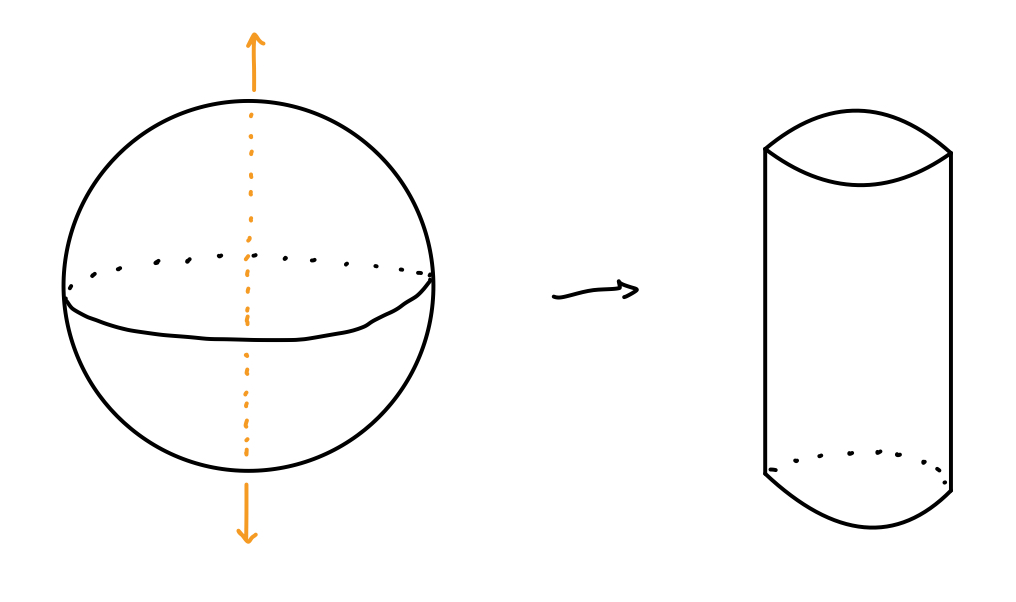
\includegraphics[scale=.2]{2-1.jpg} \end{center}
  \par With this same logic, any other lines through the sphere will have 2 intersection points, which create holes in the cylinder. 
  Thus we end up with a cylinder with $2(n-1)$ holes in it. 
  \par \begin{center} 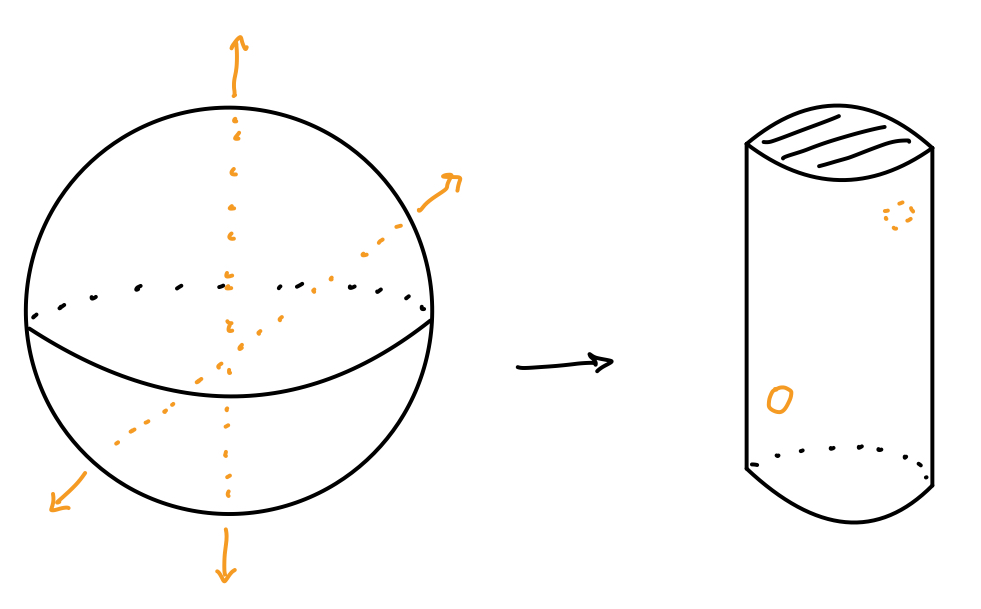
\includegraphics[scale=.2]{2-2.jpg} \end{center}
  \par These holes can be expanded, so that we end up with a cylinder with no surface, just $2(n-1)$ lines connecting the top and bottom circles.
  \par \begin{center} 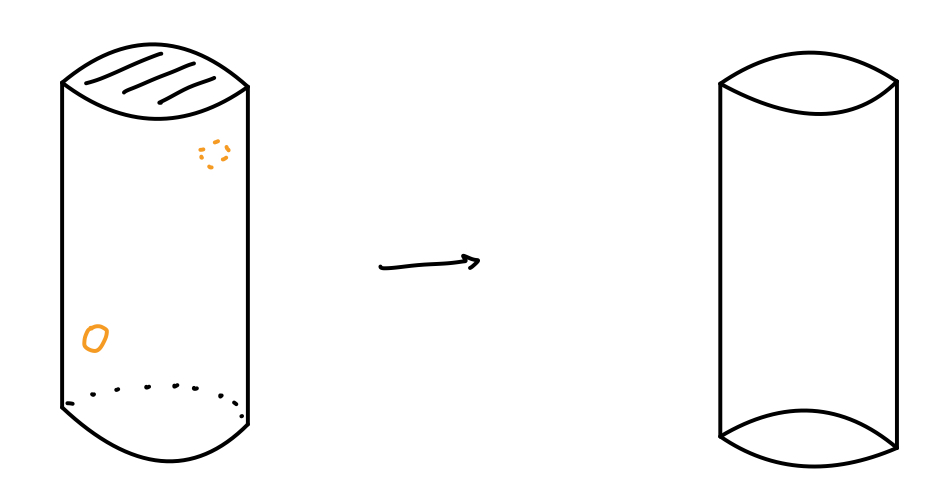
\includegraphics[scale=.2]{2-3.jpg} \end{center}
  \par One of the lines can be contracted to a point, giving us $2(n-1)$ loops with a line connecting them.
  \par \begin{center} 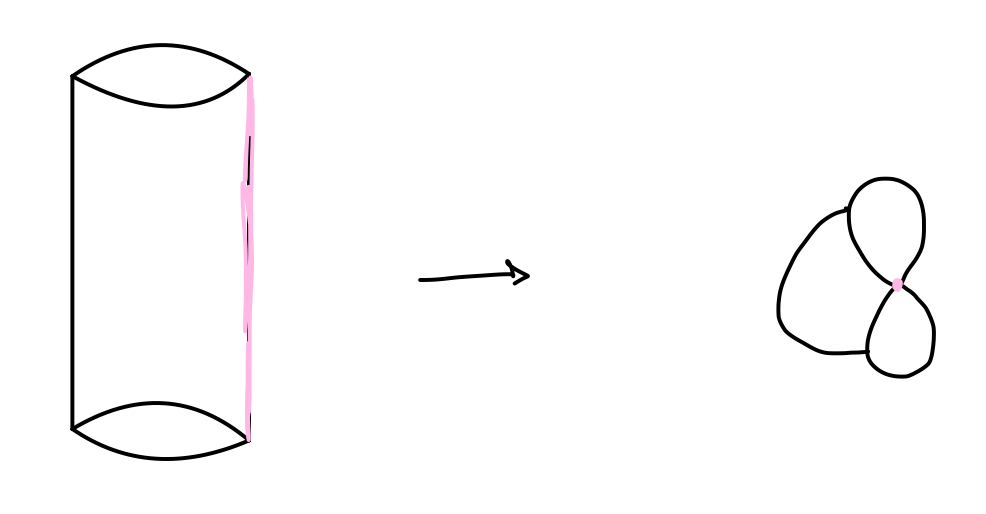
\includegraphics[scale=.2]{2-4.jpg} \end{center}
  \par This last line can be contracted to a point, and so we end up with $2(n-1)+1=2n-1$ $S^1$'s connected at a point.
  \par \begin{center} 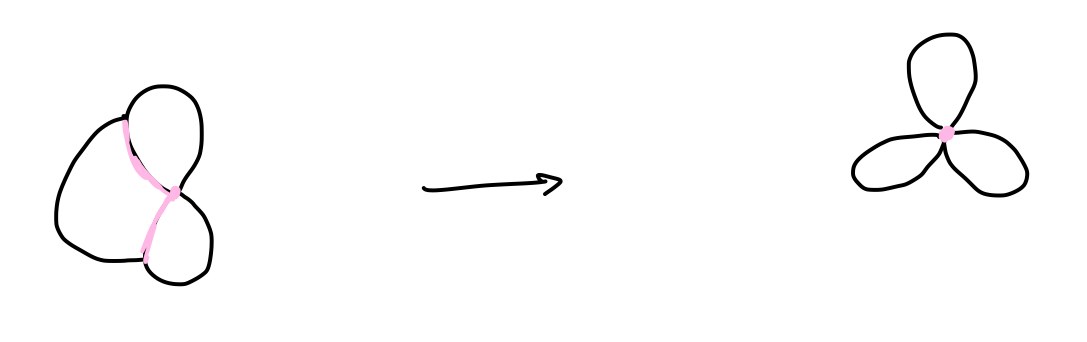
\includegraphics[scale=.2]{2-5.jpg} \end{center}
  \par Thus we have 
  \begin{align*}
    \pi_1(\mathbb{R}^3-X) & \cong \pi_1(\vee^{2n-1}(S^1)) \\
                          & \cong \pi_1(S^1) \ast \dots \ast \pi_1(S^1) \\
                          & \cong \mathbb{Z} \ast \dots \ast \mathbb{Z}
  \end{align*}
  \par And so $\mathbb{R}^3 -X$ has a fundamental group that is isomorphic to $2n-1$ copies of $\mathbb{Z}$.
\end{proof}

\begin{statement}[Problem]{3}
  Let $X$ be the quotient space of $S^2$ obstained by identifying the north and south poles to a single point. Put a cell complex structure on 
  $X$ and use this to compute $\pi_1(X)$.
\end{statement}
\begin{proof}
  When we identify these two poles, we create the following shape:
  \par \begin{center} 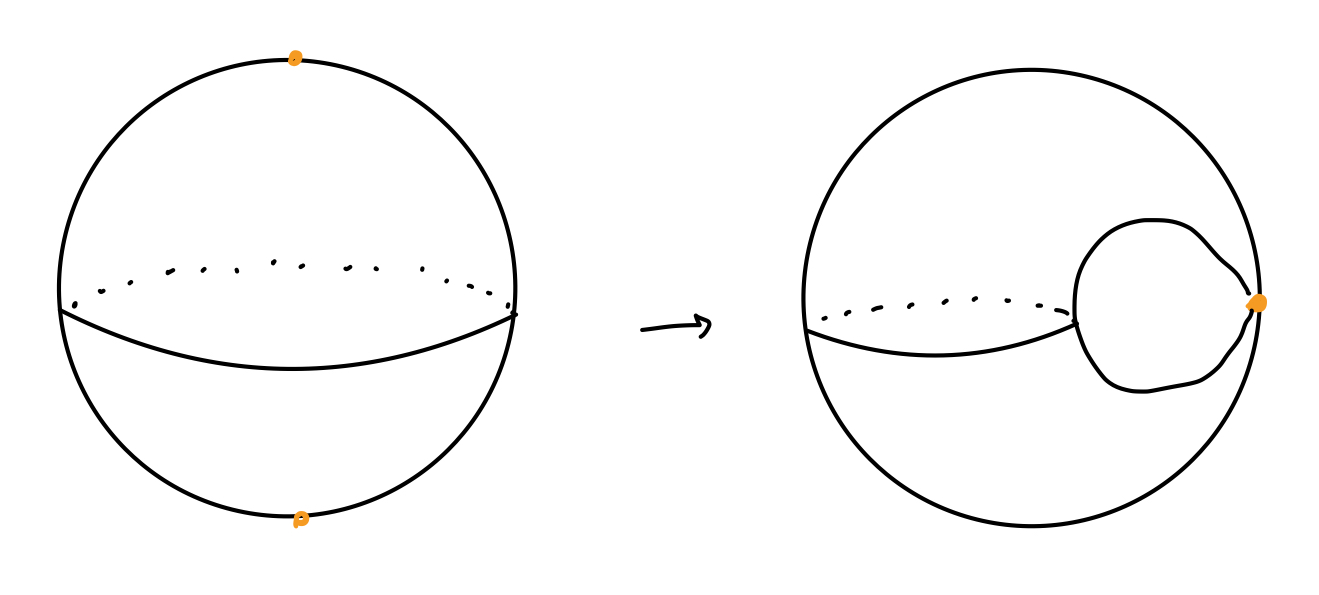
\includegraphics[scale=.2]{3-1.jpg} \end{center}
  \par We can take this point and expand it into a line
  \par \begin{center} 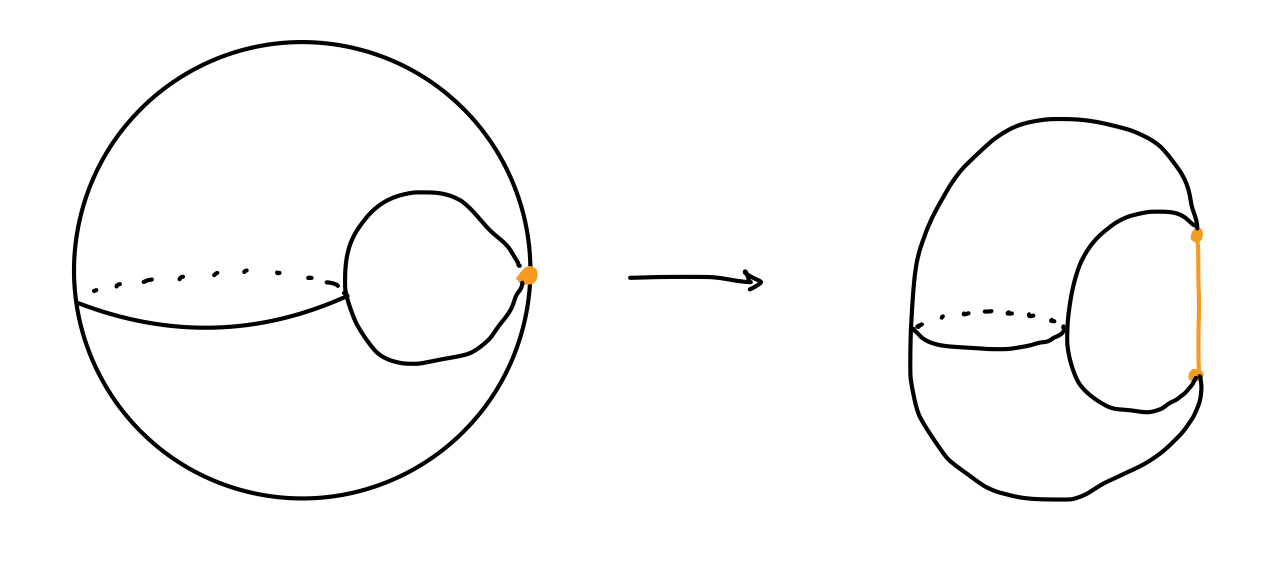
\includegraphics[scale=.2]{3-2.jpg} \end{center}
  \par Then we can take the line on the boundary of the sphere and contract it to a point, creating a loop on the outside.
  \par \begin{center} 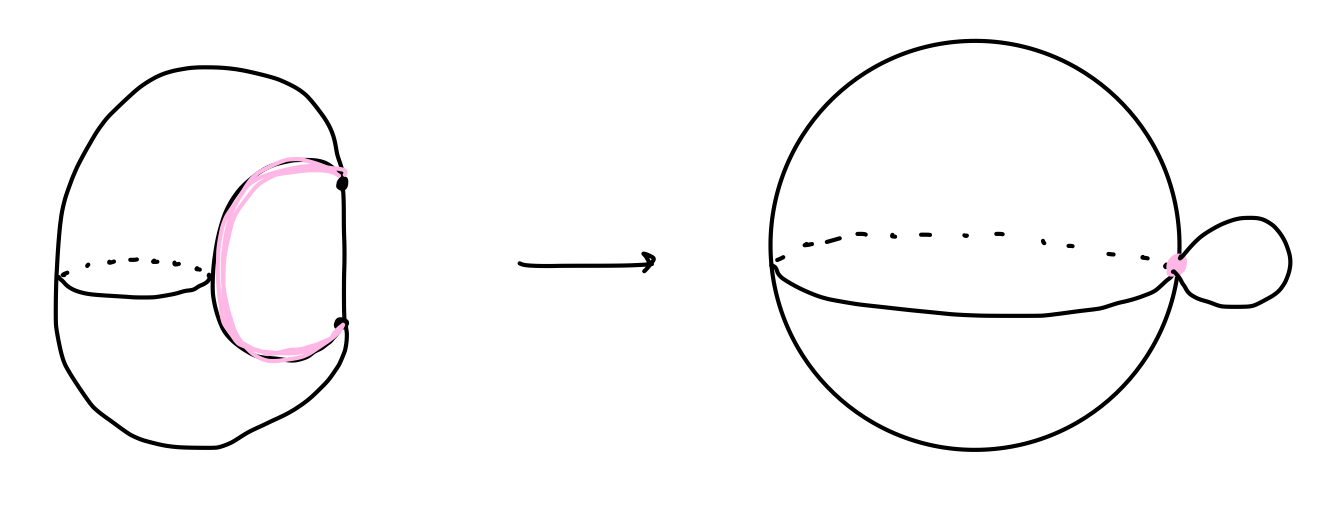
\includegraphics[scale=.2]{3-3.jpg} \end{center}
  \par Thus we have $S^2 \vee S^1$, and in terms of cell complex, an $e^0_2$ attached to an $e_1^0$ at an $e_0^0$.
  Thus the space's fundamental group can be calculated to be $0 \ast \mathbb{Z} \cong \mathbb{Z}$.
\end{proof}

\begin{statement}[Problem]{4}
  Compute the fundamental group of the space obtained from two tori $S^1 \times S^1$ by identifying a circle $S^1 \times \{x_0\}$ 
  in the torus with the corresponding circle $S^1 \times \{x_0\}$ in the other torus.
\end{statement}
\begin{proof}
  First, to get an idea of what the shape looks like, we can start with two tori in the following sense:
  \par \begin{center} 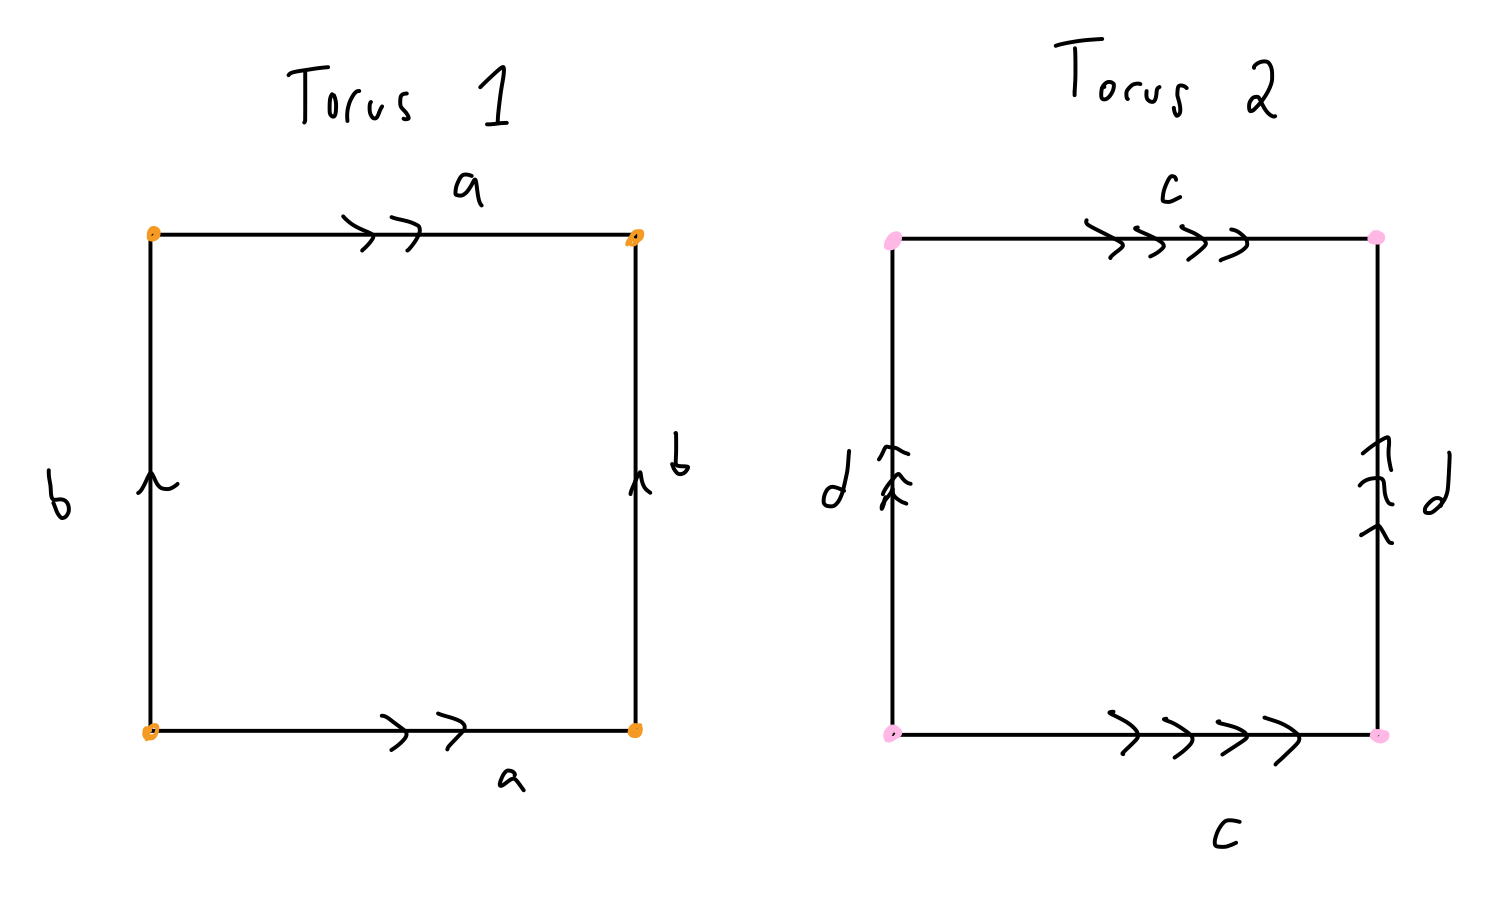
\includegraphics[scale=.2]{4-1.jpg} \end{center}
  \par When identifying one circle with another, it is equivalent to say that $b=d$. Thus the diagram transforms into this:
  \par \begin{center} 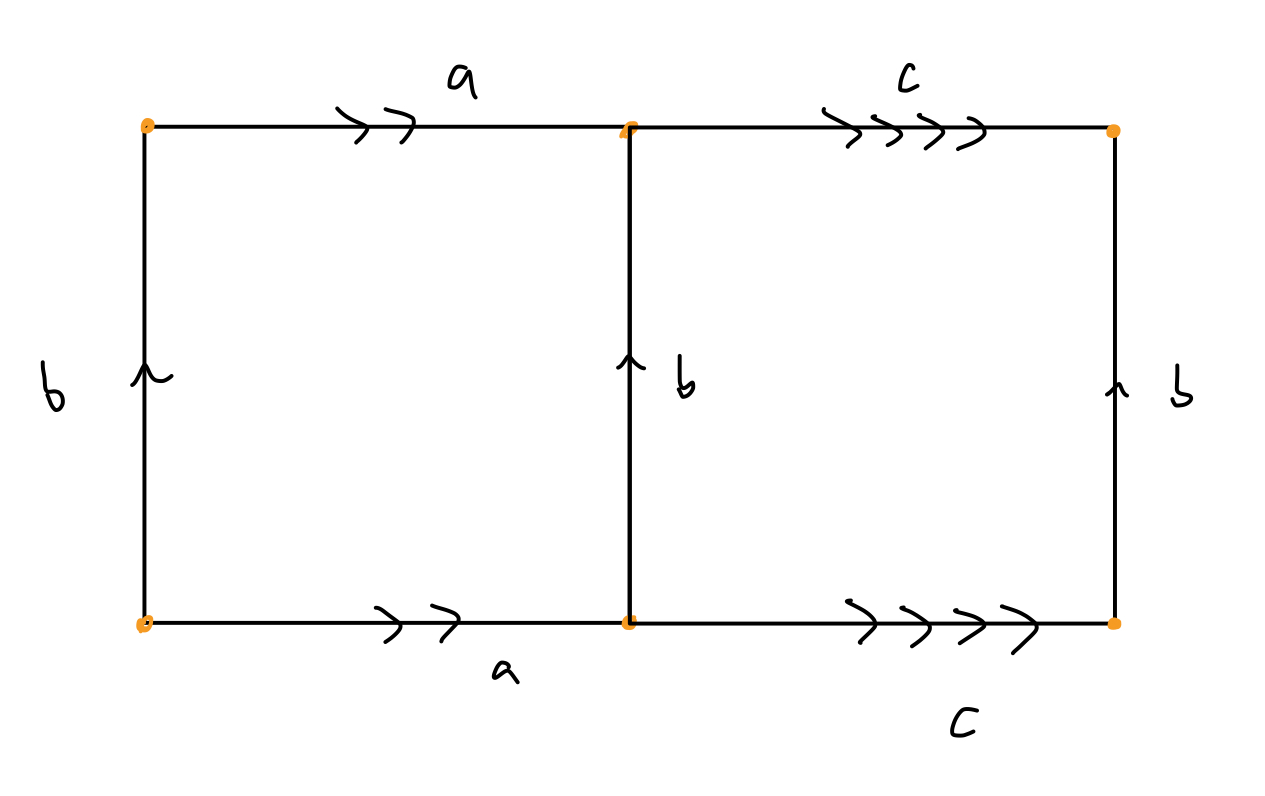
\includegraphics[scale=.2]{4-2.jpg} \end{center}
  \par Now, all 6 points are identified to each other, so we can start by gluing the 4 on the corners with the 2 in the center. 
  Once this is done, we can glue the two remaining points together.
  \par \begin{center} 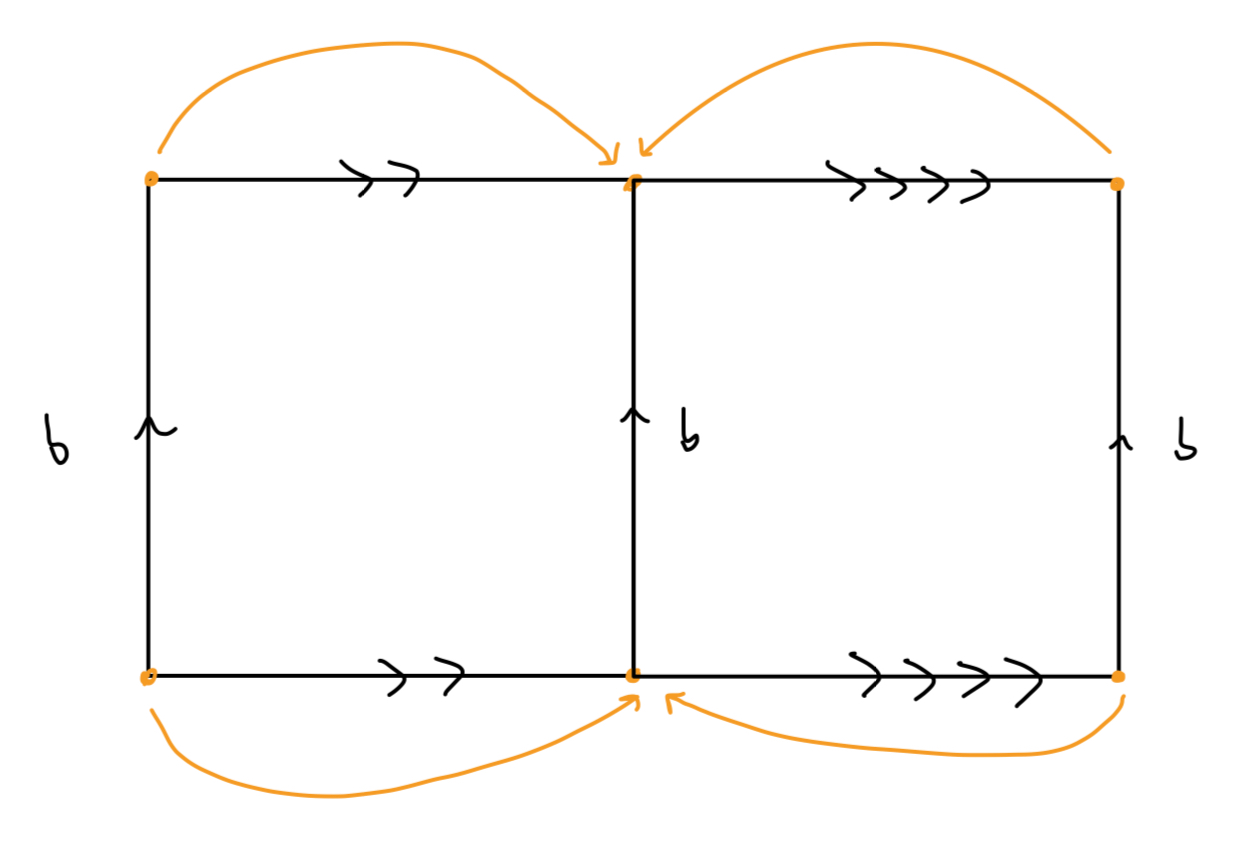
\includegraphics[scale=.2]{4-3.jpg} \end{center}
  \par \begin{center} 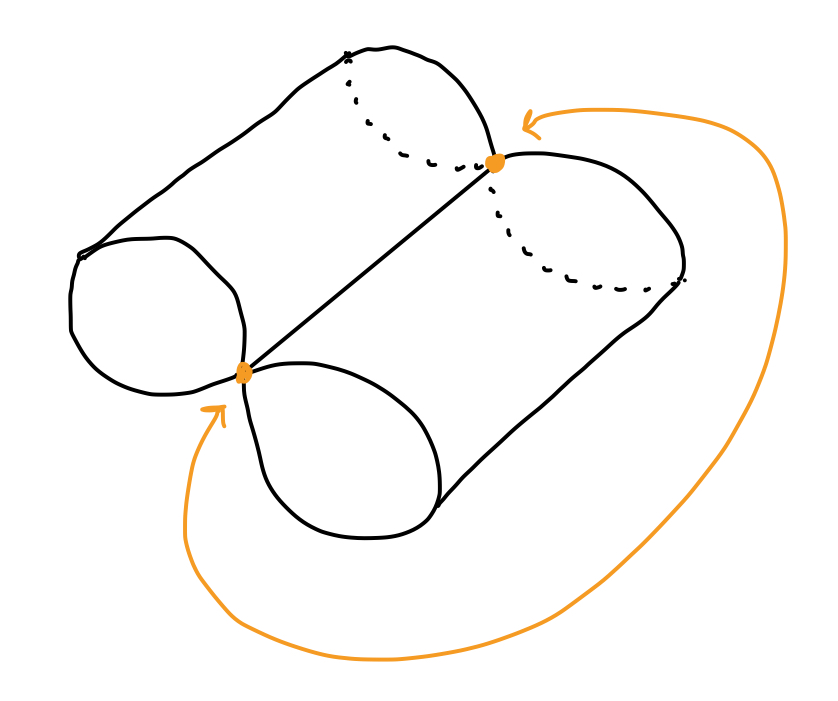
\includegraphics[scale=.2]{4-4.jpg} \end{center} 
  \par Thus we have two tori stacked on top of each other, where they only intersect on one circle on the bottom of the top one, and on the top of the bottom one. 
  \par \begin{center} 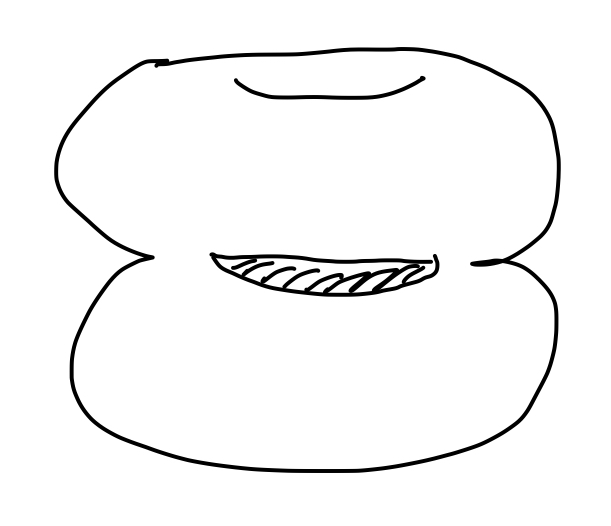
\includegraphics[scale=.2]{4-5.jpg} \end{center} 
  \par Although it may be worth considering trying this problem with Van Kampen, where the two spaces are each a torus with the intersection circle and an open neighborhood around it, it 
  may prove simpler to look at the group presentation. If we can define each separate torus like so 
  \begin{align*}
    & \pi_1(T_1) = \{a,b \text{ }|\text{ } aba^{-1}b^{-1} = 1\} \\
    & \pi_1(T_2) = \{c,d \text{ }|\text{ } cdc^{-1}d^{-1} = 1\},
  \end{align*}
  \par then, as we saw in the second diagram for this problem, we are simply asked to set $b=d$. Thus the group reprsentation for this space is 
  \begin{equation*}
    \pi_1(X) = \{a,b,c,d \text{ }|\text{ } aba^{-1}b^{-1} =1, cdc^{-1}d^{-1} = 1, b=d \}
  \end{equation*}
  \par An even simpler way to think about it would be looking at the picture; it is simply another product like the torus, but 
  instead of $S^1$ being crossed with another $S^1$, its a wedge sum of two $S^1$'s. A visual reprsentation of this is below: 
  \par \begin{center} 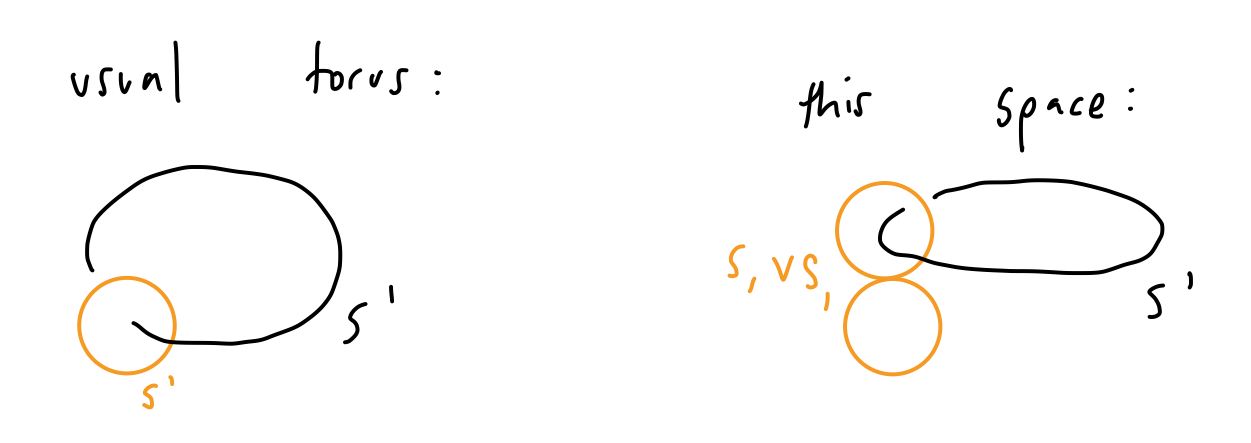
\includegraphics[scale=.2]{4-6.png} \end{center} 
  \par Thus we can conlude:
  \begin{align*}
    \pi_1(X) & \cong \pi_1(S^1 \times (S^1 \vee S^1)) \\
             & \cong \pi(S^1) \times \pi_1(S^1 \vee S^1) \\
             & \cong \mathbb{Z} \times (\mathbb{Z} \ast \mathbb{Z})
  \end{align*}
\end{proof}

\begin{statement}[Problem]{5}
 The mapping torus $T_f$ of a map $f:X \to X$ is the quotient of $X \times I$ 
 obtained by identifying each point $(x,0)$ with $(f(x),1)$. In the case $X = S^1 \vee S^1$ with $f$ basepoint-preserving,
 compute a presentation for $\pi_1(T_f)$ in terms of the induced map $f_*: \pi_1(X) \to \pi_1(X)$. Do the same when $X = S^1 \times S^1$.
\end{statement}
\begin{proof}
  When considering this as a cell complex, we can imagine the two $S^1$'s as $A$ and $B$, intersecting at a basepoint $x_0$. Let 
  $C$ be the 1-cell going around the mapping torus that maps the basepoint to itself (because $f$ is basepoint-preserving).
  Then we can define the following $2$-cells:
  \par \begin{center} 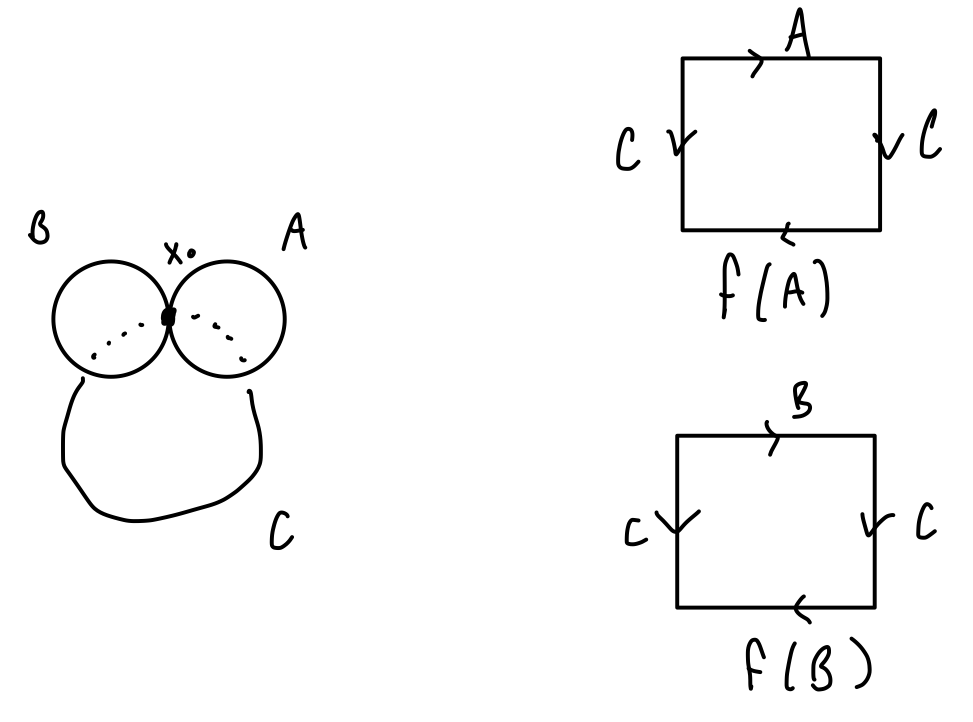
\includegraphics[scale=.2]{5-1.png} \end{center} 
  \par Thus resulting in the following presentation for the fundamental group:
  \begin{align*}
  \pi_1(X) \cong \{ a,b,c \text{ }|\text{ } acf_*(a)c^{-1}=1, bcf_*(b)c^{-1}=1  \}.
  \end{align*}
  \par When $X=S^1 \times S^1$, we're just doing a mapping torus of a torus. We can do something similar, where one point of the torus (the basepoint)
  stays constant so we can sttach a 1-cell in a loop there.
  \par \begin{center} 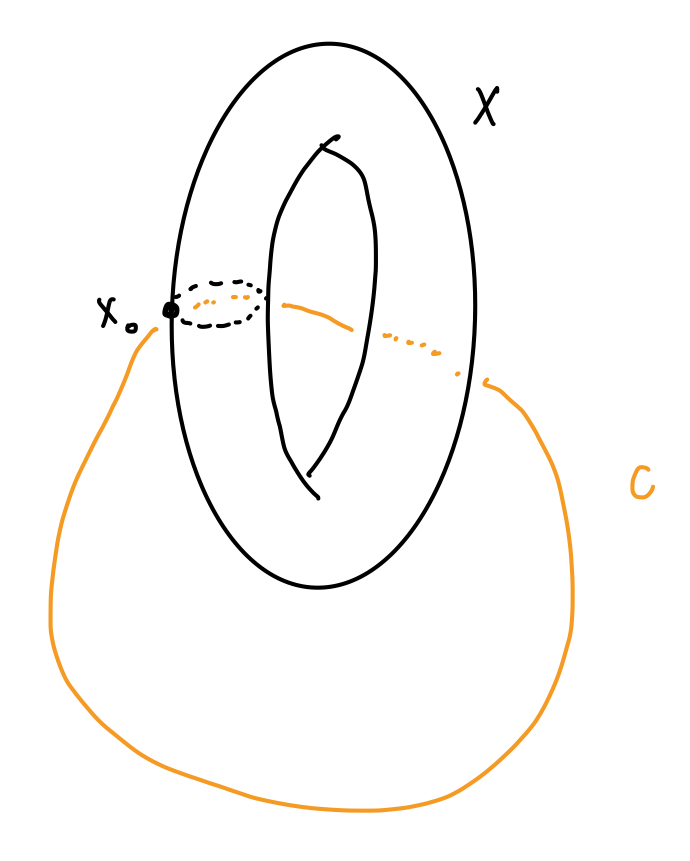
\includegraphics[scale=.2]{5-2.jpg} \end{center} 
  \par We can now attach a 3-cell along the edge of $C$, so that it is glued to $X ,f(X)$ and $C$. Thus the group presentation is 
  \begin{align*}
    \pi_1(X) \cong \{ a,c \text{ }|\text{ } acf_*(a)c^{-1}=1 \}.
  \end{align*}
\end{proof}

\end{document}
